
\graphicspath{ {3chapterTheory/image/} }
\chapter{Theoretical Background}
\section{Mathematical morphology} \label{MM}
%------------------------------------------------------------
%--------
%------------------------------------------------------------
Morphology come from Greek and means the \textit{study of shape}. Mathematical Morphology deals with describing shapes based on the set theory, integral geometry and lattice algebra. It is not just a theory but is now part of classical powerful image processing techniques. In the field of document image processing and analysis, where the shape of objects contains prominent features, some morphological operators are widely used. Mathematical morphology contains non-linear operators that can transform the shape of objects, thus allowing to extract them. The morphological operators can be classified as follows:
\begin{enumerate}
\item \textbf{Operators on binary images based on structuring element}. These operators describe the interaction of an image with a structuring element S. With $\Omega$ denote the image domain, a binary image $1_F$: $ \Omega \rightarrow \mathbb{B} $ is the indicator function of a set of point F which is a subset of an Euclidean space $ \mathbb{R}^d $ or the integer grid $\mathbb{Z}^d$ of dimension d. A structuring element is a set \textit{S}, which is usually centered in a limited definition domain, acts like a filter for any transform applying to \textit{F}. The size of S, which is usually small relative to the images, affects the strength of the transform and its sharp defines how the transform modify the shape of components in image. Many morphological operators have been defined, some of them are dual by set complementation. Two basic morphology operators, erosion and dilation, belong to this class. Erosion is defined as $ \epsilon_S (F) = \lbrace p  \vert  \forall s \in S, p + s \in F\rbrace $  and dilation is defined as $ \delta_S (F) = \lbrace p+s  \vert  \forall p \in F, s \in S\rbrace $ Their effects can be seen in Figure \ref{fig:erosionbin} and  Figure \ref{fig:dilationbin}. They are dual operators with respect to complementation $ \epsilon_S (F) = \overline{\delta_{S} \overline{F}} $ . This duality property illustrates the fact that erosion and dilation do not process the objects and their background symmetrically: the erosion shrinks the objects but expands their background (and vice versa for the dilation).
\par Other interesting morphological filters can be formed using the differences of two or more operators, for example the morphological gradient and morphological Laplacian. As the erosion shrinks objects and the dilation grows them, examining the difference between original image and its erosion and dilation can give us information of the edge of objects. The morphological gradient is defined by $\triangledown_S (F) = \delta_S (F) - \epsilon_S (F) $. This thick gradient appears on two sides of the acture edges and can be decomposed into two half gradient $\triangledown_S (F) = \triangledown_S ^- (F) + \triangledown_S ^+ (F)$ with $ \triangledown_S ^- (F) = F - \epsilon_S (F)$ is the inner gradient adheres to insides of objects and $ \triangledown_S ^+ (F) =\delta_S (F) - F$ is the outer gradient, adheres to the outside of objects. The morphological equivalent of the Laplacian is defined by $\vartriangle_S (F) =\triangledown_S ^+ (F) - \triangledown_S ^- (F)=\delta_S (F)+\epsilon_S (F) - 2F$. An example of these operators are shown in Figure \ref{fig:gradientbin}, Figure\ref{fig:gradientInbin}, Figure \ref{fig:gradientOutbin} and Figure \ref{fig:laplacianbin}

\begin{figure}
	\begin{subfigure}{0.2\textwidth}
	 	
\includegraphics{bin/input.png} \caption{Input F}\label{fig:inputbin} \end{subfigure}
	\begin{subfigure}{0.2\textwidth}
	 	
\includegraphics{bin/erosion.png} \caption{$ \epsilon_S (F)$}\label{fig:erosionbin} \end{subfigure}
	\begin{subfigure}{0.2\textwidth}
		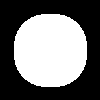
\includegraphics{bin/dilation.png} \caption{$ \delta_S (F)$}\label{fig:dilationbin} \end{subfigure}
	\centering
		
	\begin{subfigure}{0.2\textwidth}
		
\includegraphics{bin/gradient.png} 
		\caption{$ \triangledown_S (F)$}\label{fig:gradientbin} \end{subfigure}
	\begin{subfigure}{0.2\textwidth}
		
\includegraphics{bin/gradientIn.png} 
		\caption{$ \triangledown_S ^- (F)$}\label{fig:gradientInbin} \end{subfigure}		
	\begin{subfigure}{0.2\textwidth}	
		
\includegraphics{bin/gradientOut.png} 
		\caption{$ \triangledown_S ^+ (F)$}\label{fig:gradientOutbin} \end{subfigure}
	\begin{subfigure}{0.2\textwidth}	
		
\includegraphics{bin/laplacian.png} 
		\caption{$\vartriangle_S (F)$}\label{fig:laplacianbin} \end{subfigure}					
	\centering
	\caption[Example of \textit{morphological operators} on binary image] {Binary Morphological operators. The morphological Laplacian is colorized by Green (positive), red (negative) and black (zero) }
	\label{fig:binOperations}
\end{figure}


\item \textbf{Elementary operators of binary images on sets}. By replacing the structuring element B by the notion of neighborhood $\mathcal{N}$, morphological operators obtained will have elementary behavior (the slightest transform effect possible). For example, $ \delta_\mathcal{N} (F) = \lbrace p' \in \mathcal{N}(p) \cup p  \vert  p \in F \rbrace $ is the elementary dilation.

\item \textbf{Extension from sets to functions of the first two categories}. Applying threshold decomposition principle, morphological operators can be extended to function i.e. gray level images. $ f: \Omega \rightarrow \mathbb{N}$. With a given gray level $t$, the subset of $ \Omega $ obtained by thresholding f by t is denoted by $[f \geq t] = \lbrace p \in \mathcal{D} \vert f(p) \geq t \rbrace $. Any morphological set operator $\phi^{set}$ can be extended to define a morphological operator on gray level function $\phi$ using $ \phi(f)(p) = max \lbrace t \vert p \in \phi^{set}([f \geq t]) \rbrace $. Illustrations of these operators are given in Figure \ref{fig:grayLevelOperations}.

\begin{figure}
	\begin{subfigure}{0.2\textwidth}
	 	
\includegraphics{grayLevel/input.png} \caption{Input F}\label{fig:inputgrayLevel} \end{subfigure}
	\begin{subfigure}{0.2\textwidth}
	 	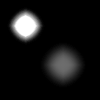
\includegraphics{grayLevel/erosion.png} \caption{$ \epsilon_S (F)$}\label{fig:erosiongrayLevel} \end{subfigure}
	\begin{subfigure}{0.2\textwidth}
		
\includegraphics{grayLevel/dilation.png} \caption{$ \delta_S (F)$}\label{fig:dilationgrayLevel} \end{subfigure}
	\centering
		
	\begin{subfigure}{0.2\textwidth}
		
\includegraphics{grayLevel/gradient.png} 
		\caption{$ \triangledown_S (F)$}\label{fig:gradientgrayLevel} \end{subfigure}
	\begin{subfigure}{0.2\textwidth}
		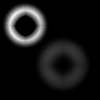
\includegraphics{grayLevel/gradientIn.png} 
		\caption{$ \triangledown_S ^- (F)$}\label{fig:gradientIngrayLevel} \end{subfigure}		
	\begin{subfigure}{0.2\textwidth}	
		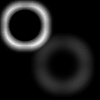
\includegraphics{grayLevel/gradientOut.png} 
		\caption{$ \triangledown_S ^+ (F)$}\label{fig:gradientOutgrayLevel} \end{subfigure}
	\begin{subfigure}{0.2\textwidth}	
		
\includegraphics{grayLevel/laplacian.png} 
		\caption{$\vartriangle_S (F)$}\label{fig:laplaciangrayLevel} \end{subfigure}					
	\centering
	\caption[Example of \textit{morphological operations} on gray level image] {Morphological operations on set, using a square 10x10 pixels as the structuring element. (The laplacian is colorized by Green (positive), red (negative) and black (zero)) }
	\label{fig:grayLevelOperations}
\end{figure}


\item \textbf{Connected operators}. Connected operators \cite{Salembier95flatzones} are operator that work by merging elementary region called flat zones. It verified 
$ \forall p, \forall p' \in \mathcal{N}(p), f(p')=f(p) \Longrightarrow  \phi(f)(p')=\phi(f)(p)$. As a consequence, connecting operators will not create contours, nor modify their positions. Therefore, they have a very good contour preservation property. There are two commonly used classes of connected operators: filters by reconstruction and algebraic openings and closings \cite{Vincent.1993.tip}. Although they are not only defined for the binary case, where only objects "marked" by another image are extracted. Connected operators are also defined for gray level images by thresholding the input image at different level t. 
\end{enumerate}
\par Mathematical morphology is a powerful tool for image processing. It found application in numerous fields: geosciences and remote sensing, materials science, biological and medical imaging, industrial applications, identification and security control, document processing and image coding \cite{Soille:2003:MIA:773286}. Some authors used basic morphological operators such as erosion, dilation, opening and closing in text detection field. For example, they use operators of the first 3 classes to group extracted strokes\cite{Zhang.2015.Neurocomputing} or edges \cite{Ye.2003.ICICS} \cite{Pillai.2013.ICCPCT} but rarely the class of connected operators. 

\section{Digital topology and self-duality}
\subsection{Basic notions of digital topology}
\par
A 2D discrete image I is a function $ \Omega \rightarrow E$ with E being a set. I is a digital binary image when $E = \lbrace0,1\rbrace$ and it is said a gray scale image when $E = \lbrace0, \dots, k\rbrace$. A point of I is a couple $p = (x,y) \in \mathbb{Z}^2$. Two point $p_1 =(x_1,y_1),p_2=(x_2,y_2)$ are:
\begin{itemize}
\item 4-adjacent if and only if $d_4 (p_1,p_2) =\vert x_1 - x_2 \vert + \vert y_1 - y_2 \vert = 1 $
\item 8-adjacent if and only if $d_8 (p_1,p_2) =max (\vert x_1 - x_2 \vert , \vert y_1 - y_2 \vert) = 1 $
\end{itemize}
\par
The n-neighborhood $N_n (p)$ of a point p is the set of all the points n-adjacent to p, with $n = 4$ or $n = 8$.
\subsection{Self-duality}
\par 
In the case of text detection in gray-scale images, a well-known problem encountered is that there exist bright texts over dark background and dark texts over bright background. Common workaround by processing both the original and it complement increases computation cost. Consequently, we are interested in the family of self-dual operators.
\par
A self-dual operation processes the image contents regardless the reverse of contrast \cite{geraud.15.ismm}. In general,  non self-dual operations do not process similarly bright objects over dark background and dark objects over bright background similarly which is often an undesirable feature. It is important when no assumption about the contrast between object and background can be made. As any part of the image could be the subject, we expect an operator which behaviors the same way regardless the contrast between the subject and its background.  
\begin{figure}

	\begin{subfigure}{0.3\textwidth}
	 	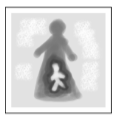
\includegraphics{im1.png} \caption{}\label{fig:gray} \end{subfigure}
	\begin{subfigure}{0.3\textwidth}
		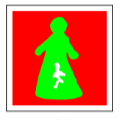
\includegraphics{im2.png} \caption{}\label{fig:mother} \end{subfigure}
	\begin{subfigure}{0.3\textwidth}
		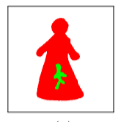
\includegraphics{im3.png} \caption{}\label{fig:baby} \end{subfigure}
	\centering
	\caption[Example of \textit{ subjects} can be either bright over dart or dart over bright] {From the original gray level image \ref{fig:gray}, the subject can be either the mother \ref{fig:mother} (dark over bright) or the baby \ref{fig:baby} (bright over dark) }
	\label{fig:motheAndBaby}
\end{figure}

\par
An example is depicted in Figure \ref{fig:motheAndBaby}. The background and foreground are respectively represented by green and red. From the grayscale image \ref{fig:gray} If we focus on the mother, then the outer zone will be the background as in Figure \ref{fig:mother}. Furthermore, we can choose the baby as the subject, therefore the woman will become the background (Figure \ref{fig:baby}).	
\par
One drawback of digital topology is the connectivity paradox related to the discrete version of the Jordan theorem. As claimed in \cite{Kong:1989:DTI:71397.71400}, if the same connectivity is used for both the object and background, the Jordan curve theorem is not respected. In order to solve this problem, a pair of connectivity is used: for an image defined in the regular cubical grid, the digital topology must be described by a "Jordan pair" of connectivity $(c_\alpha,c_\beta)$ . One connectivity is used for the dark pixels and the other one for the bright pixels. 

\par 
For example, if the image in Figure \ref{fig:topo} is describe by the pair $(c_4,c_8)$ (the 4-connectivity for background (bright pixels) and 8-connectivity for object (dark pixels)) we will obtain one object like in Figure \ref{fig:topoa}. On the same image, using $(c_8,c_4)$ gives us two separate objects (Figure (\ref{fig:topob}). This arbitrary choice affects the topology. In fact, self-dual operators must use different connectivity for the complementary to work in the same way as demonstrated in Figure \ref{fig:topoa} and Figure \ref{fig:topoc}: the complement image must use the $(c_8,c_4)$ connectivity to give the same presentation of the original image which use $(c_4,c_8)$. As no assumption is made about the gray level of the background and object, it is better to avoid the choise of connectivity. Another approach draws our attention to: the well-composed images. Latecki et al. \cite{Latecki95} present this image class which enjoys very useful topological and geometric properties, especially the fact that there is only one connectivity relationship between points of the image.

\begin{figure}

	\begin{subfigure}[b]{0.3\textwidth}
	 	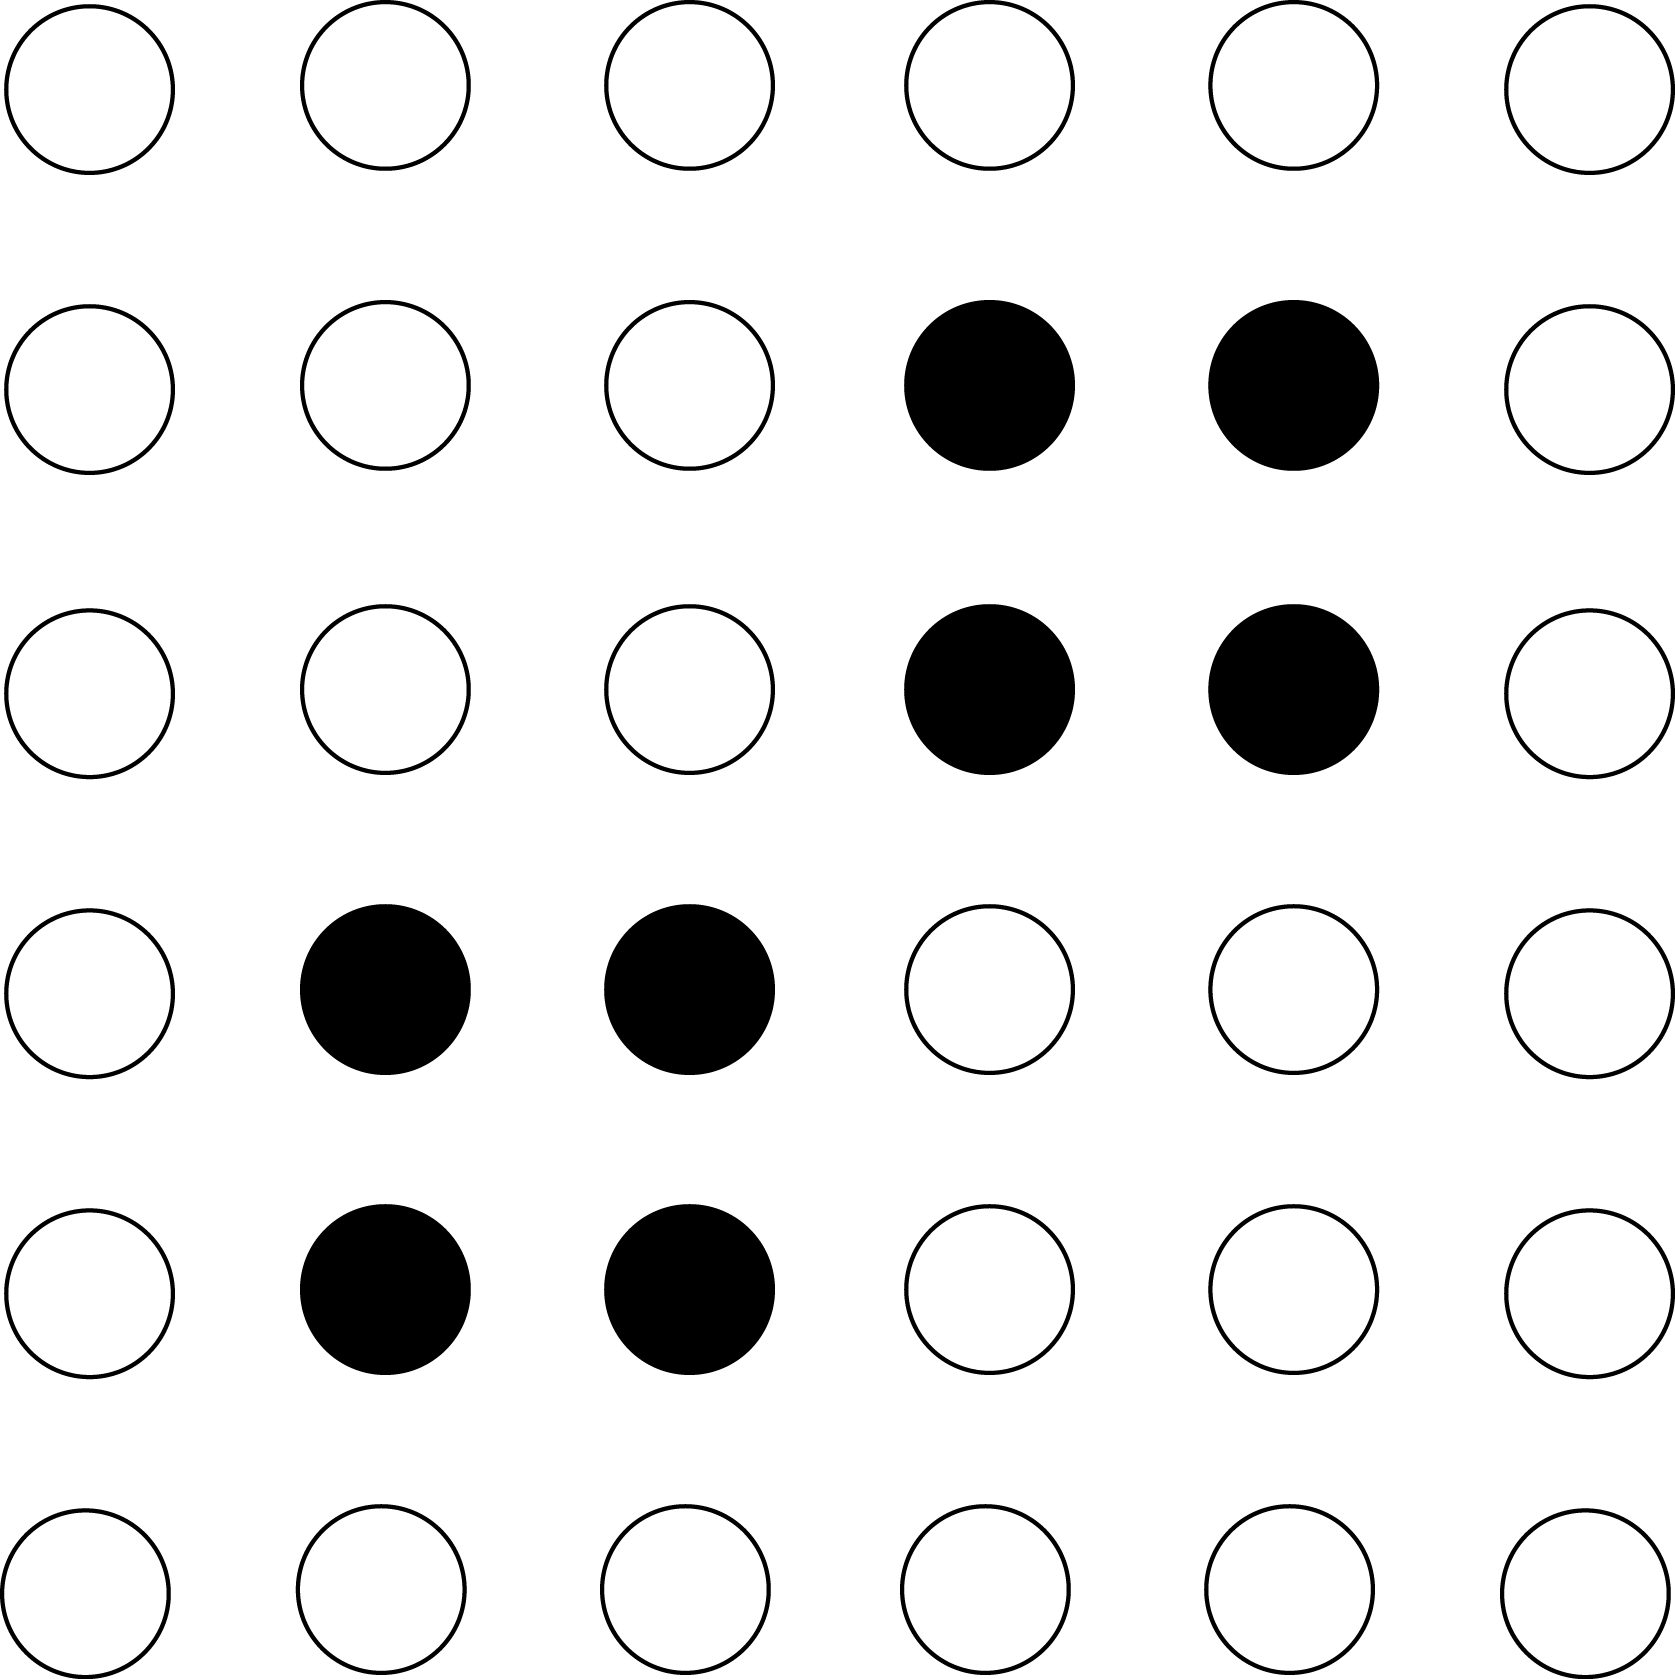
\includegraphics[width=5cm]{topo.png} \caption{}\label{fig:topo} \end{subfigure}
	\begin{subfigure}[b]{0.3\textwidth}
		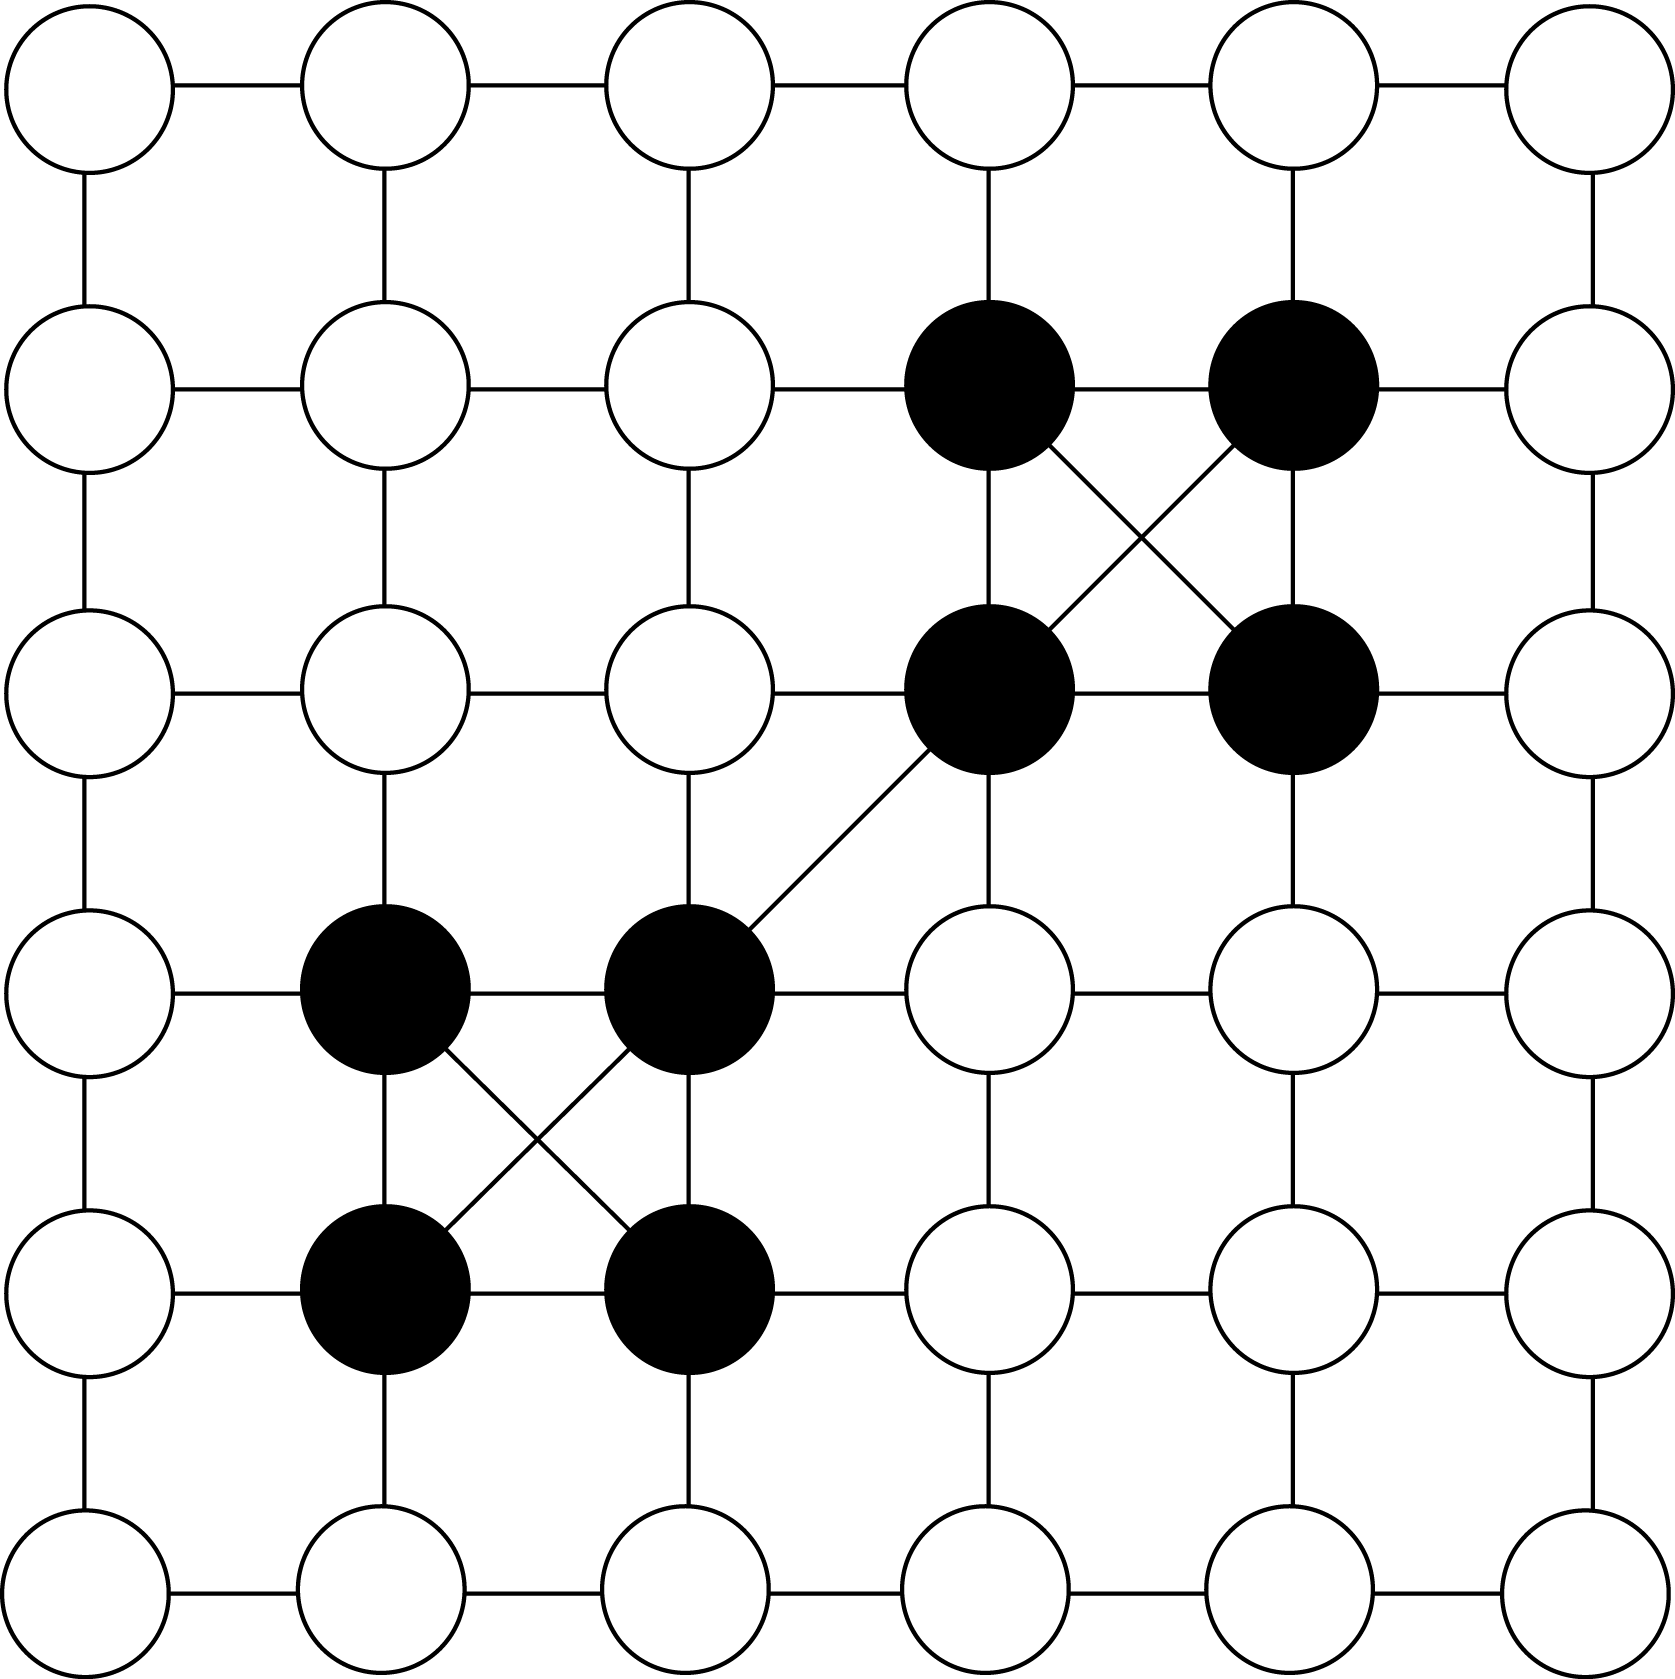
\includegraphics[width=5cm]{topoa.png} \caption{}\label{fig:topoa} \end{subfigure}	
\centering		
		
	\begin{subfigure}[b]{0.3\textwidth}
		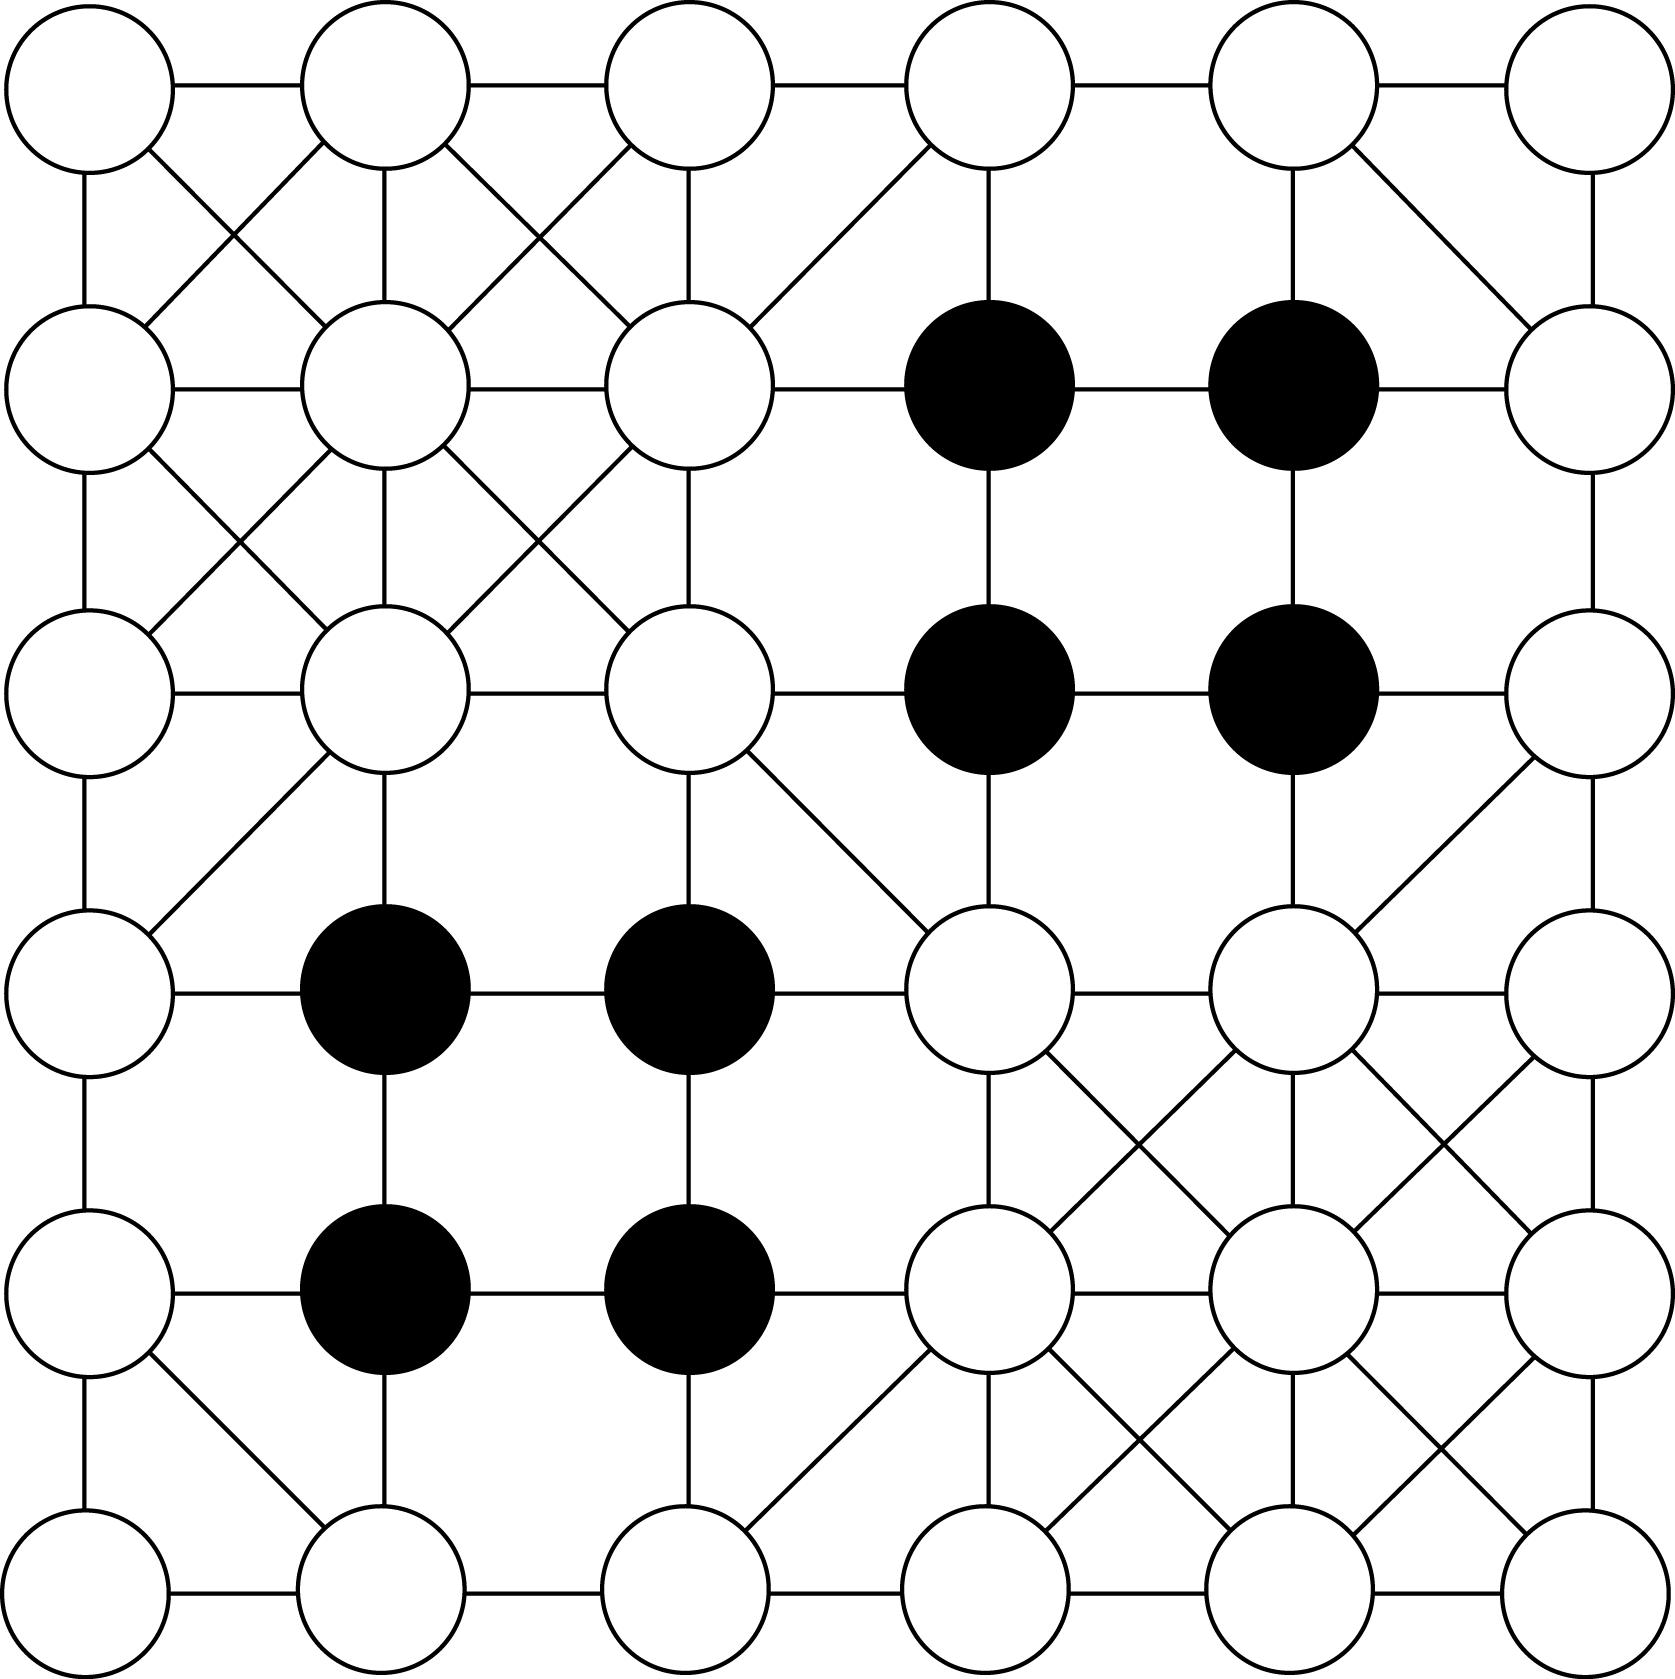
\includegraphics[width=5cm]{topob.png} \caption{}\label{fig:topob} \end{subfigure}
	\begin{subfigure}[b]{0.3\textwidth}
		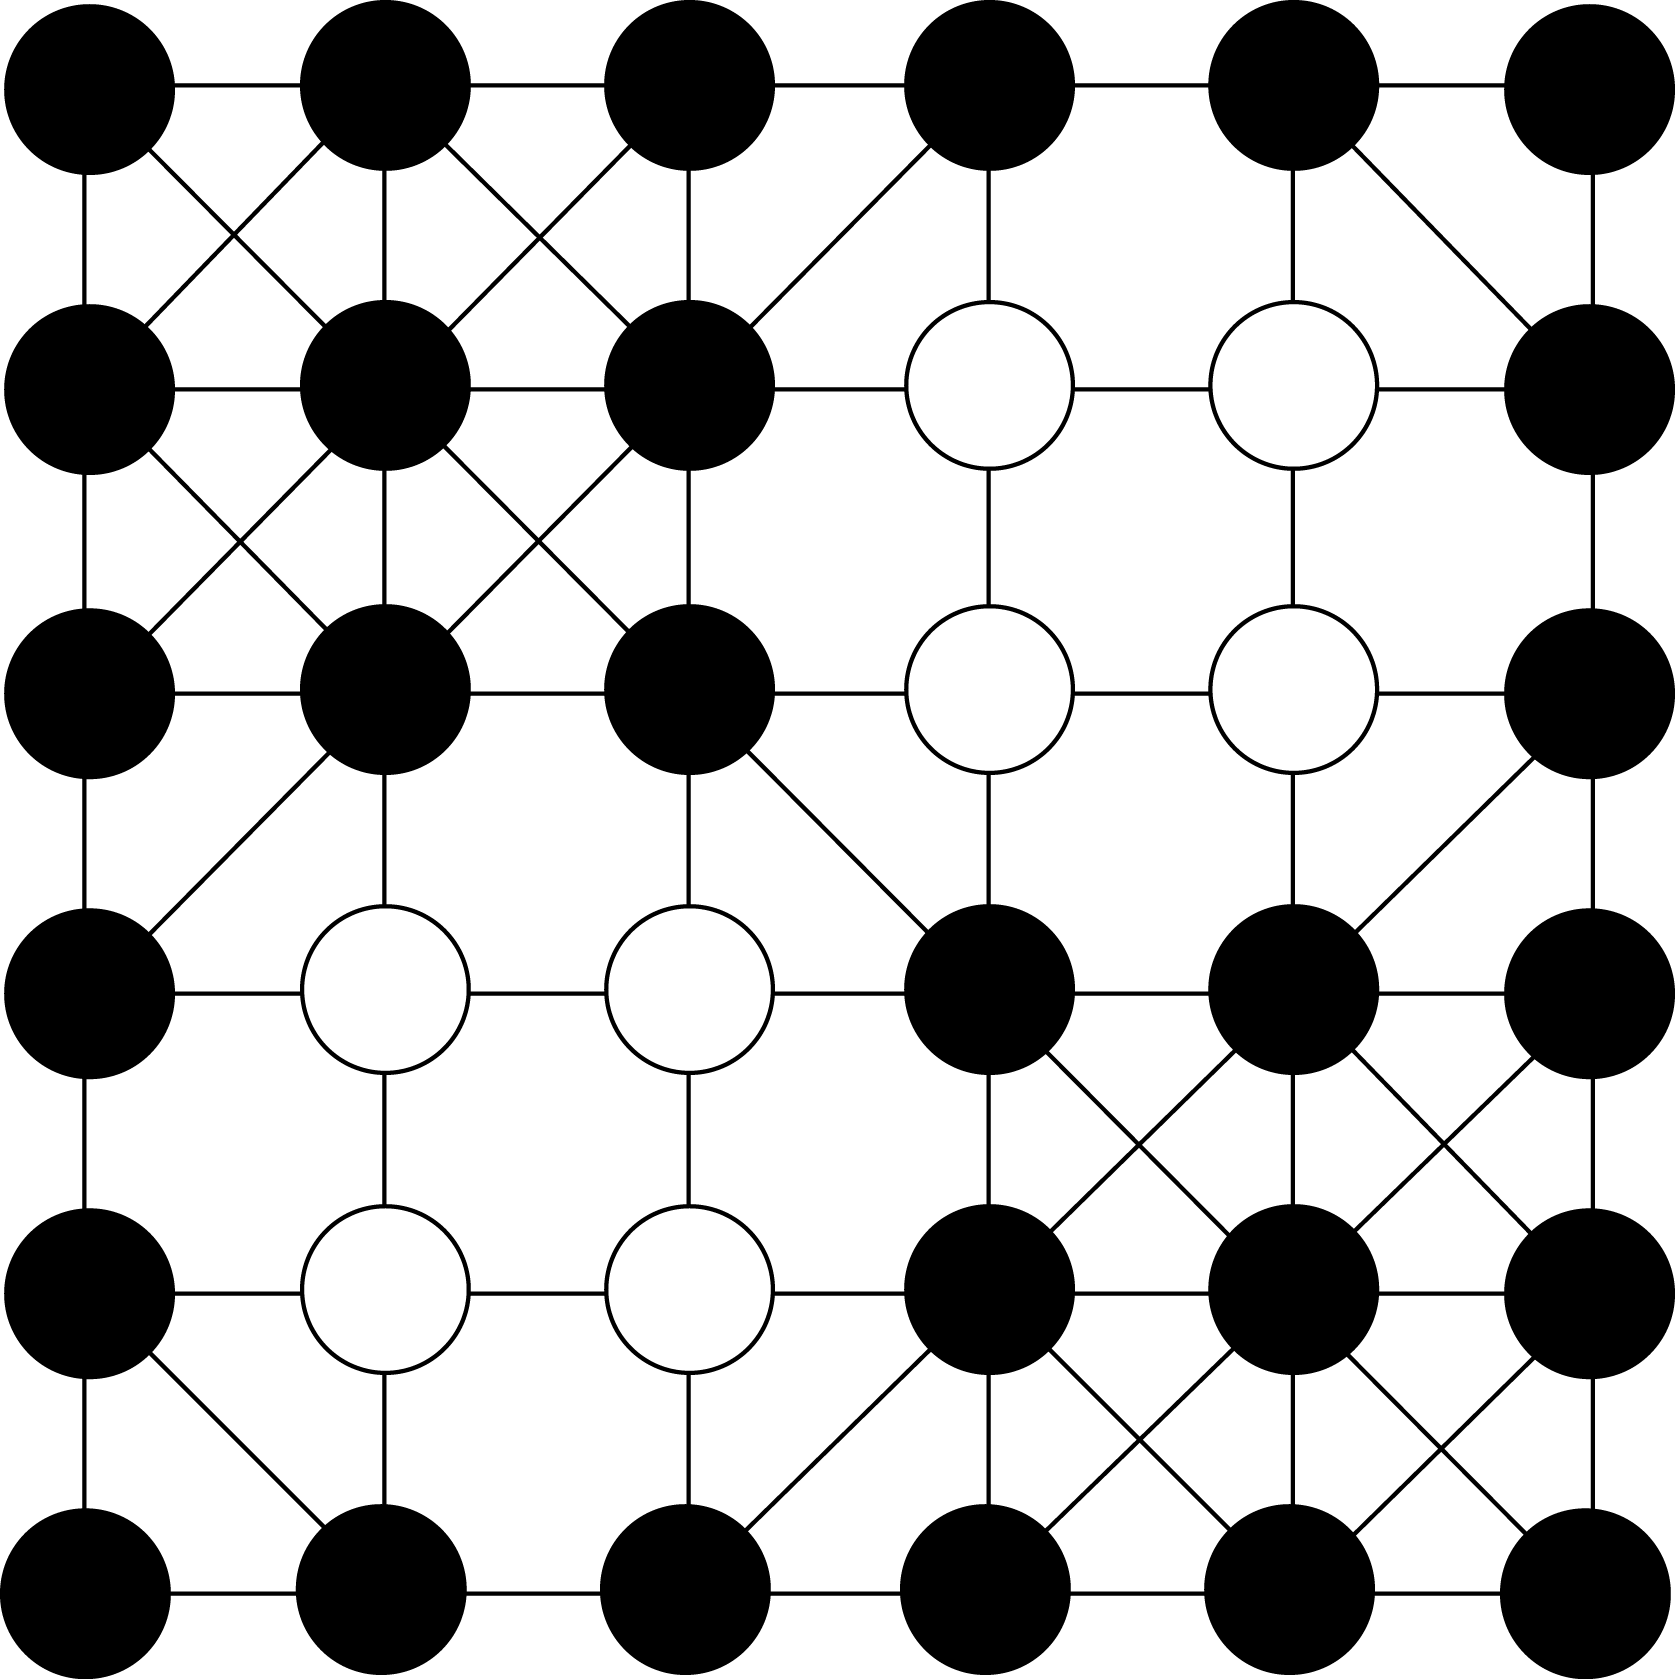
\includegraphics[width=5cm]{topoc.png} \caption{}\label{fig:topoc} \end{subfigure}
	\centering
	\caption[Example of \textit{Jordan pair} of connectivity] {Example of \textit{Jordan pair} of connectivity}
	\label{fig:Jordanpair}
\end{figure}


\section{Well-composed images} \label{Wellcomposed}
Based on the digital topology framework, notion of well-composedness has been introduced to characterize the binary images whose structure intrinsically avoids the connectivity paradox. As defined in \cite{Latecki95}, a 2D set S is weakly well-composed if any 8-component of S is a 4 component. S is well-composed if both S and its complement $\bar{S}$ are weakly well-composed. Well-composedness can be verified  using the notion of \textit{critical configurations} which are 
\includegraphics{confi1.jpg} and 
\includegraphics{confi2.jpg} : S is well-composed if these configuration do not appear. 
\par
The notion of well-composedness has also been extended to gray-level images. A gray-level image $\mu$ is well-composed if any set $[\mu \geq \lambda ]$ is well-composed. The extended version of "critical configuration" is that every block
\begin{tabular}{|c|c|}
\hline 
a & d \\ 
\hline 
c & b \\ 
\hline 
\end{tabular} 
must verify $interval(a,b) \cap interval(c,d) \neq \varnothing$ , where $interval(a,b) = [min(a,b),max(a,b)]$.
\par
Latecki has shown in \cite{Latecki.98.JMIV} that a topology preserved digitization process must result in a well-composed image. An image, especially lossy compressed one, is not \textit{a priori} well-composed. Furthermore, as only one type of connectivity is used so no choice of connectivity pair is needed. In consequence, self-dual operation can be defined without any arbitrate choice. This properties has motivated the development of algorithms to make an image well-composed. There are currently 2 approaches to get a well-composed image from the original image: by changing its pixel value (with the possibility of alter the image's topology) or by a well-composed interpolation \cite{theo.2014}.


\section{Connected operators and morphological tree}
\subsection{Connected operators}
Motivated by families of filters by reconstruction, the notion of connected operators is introduced in \cite{Salembier95flatzones} \cite{Serra1993}. As said in \ref{MM}, connected operators works by simplifying the images. The most important feature of this type of operator is preservation of contours \cite{Salembier2009}: they does not create new contours nor shift them. 
\subsection{Morphological Tree-Based Image Representation}
One popular strategy to define connected operators relies on a hierarchical region-based representation of the input image, in another word, a tree. The filtering step is achieved by pruning that tree and the output image is reconstructed from the pruned tree.  Tree of shapes is a contrast-invariant image representation which is defined in \cite{Monasse.2000}.
\paragraph{} \textbf{A Couple of Dual Trees}: given an image $\mu $ in nD: $\Omega \rightarrow \mathbb{Z} $, the lower cuts of $\mu$ are defined by 
	$[\mu < \lambda] =\lbrace x \in \Omega \vert \mu (x) < \lambda \rbrace $. The set of all connected components of all these cuts is $ \mathcal{T}_< (\mu) =\lbrace \Gamma \in \mathcal{C}\mathcal{C}([\mu < \lambda]) \rbrace $ (with $\mathcal{C}\mathcal{C}$ denote the operator that takes a set and gives its set of connected component. As these CC verify $\forall \Gamma$ and $\Gamma ' \subset \Gamma$, $\Gamma \subset \Gamma ' $ or $\Gamma \cap \Gamma '= \emptyset$, they can be arranged into a tree, called the \textit{min-tree} (because it if form using lower cuts, and the leaves will be minimum of image). We can also consider the upper cuts $[\mu \geq \lambda] =\lbrace x \in X \vert \mu (x) \geq \lambda \rbrace $, the element of $ \mathcal{T}_\geq (\mu) =\lbrace \Gamma \in \mathcal{C}\mathcal{C}([\mu \geq \lambda]) \rbrace $ will be organized into the \textit{max-tree}. The \textit{max-tree} and \textit{min-tree} are dual by complementation, the max-tree of $\mu$ is the min-tree of $ \mu$, therefore operators defined on them are dual.
	
\paragraph{} \textbf{A Self-Dual Tree}:We use two sets $ \mathcal{T}_< (\mu)$ and $ \mathcal{T}_\geq (\mu)$ with their holes filled to define two other sets $ \mathcal{S}_< (\mu)$ and $ \mathcal{S}_< (\mu)$. We denote \textit{Sat} as the cavity-fill-in operator, these new sets are defined as: $ \mathcal{S}_< (\mu) = \lbrace Sat(\Gamma);\Gamma \in \mathcal{T}_<(\mu)\rbrace$ and $ \mathcal{S}_\geq (\mu) = \lbrace Sat(\Gamma);\Gamma \in \mathcal{T}_\geq (\mu)\rbrace$. The tree of shape is defined as: $\mathfrak{S}(\mu) = \mathcal{S}_< (\mu) \bigcup \mathcal{S}_\geq (\mu) $. We have also $\Gamma \subset \Gamma ' $ or $\Gamma \cap \Gamma '= \emptyset$ with $\Gamma , \Gamma ' \in \mathcal{S}$. There is a quasi-linear algorithm to compute the tree of shape, which works also in the case of nD presented in \cite{geraud.13.ismm}. This tree is \textit{self-dual} because many self dual operation can be defined in this tree. \fxnote{re read theo paper}

The min and max tree are easily compute with a few line of code \cite{berger.07.icip} and the tree of shape can be obtain thanks to \cite{geraud.13.ismm}. The tree encoding is very compact in term of memory: the parenthood relationship between pixels is an image having the same size of the input. 

\subsection{Some application}
The connected operators are attractive in applications where the image has to be simplified without losing information about the contours. A large number of simplification criteria such as size, area, contrast or complexity can be obtained with these operator. They found application in image simplification and segmentation.